\documentclass[a4paper, 12pt]{article}
\usepackage[UTF8]{ctex}
% \usepackage[T1]{fontenc}
% \usepackage{inconsolata}


\usepackage{amsmath}
\usepackage{enumitem}
\setlist{
    nolistsep, % 去掉 item 和正文之间的间隔
    % labelindent=\parindent,
    leftmargin=*, % 保证小节标签缩进和上面对齐
    % labelsep=1em, % 标签后的空白
    align=left, % 标签对齐段落左边缘
}
\usepackage{tabularx}

\usepackage{graphicx}

\usepackage{geometry}
\geometry{
    a4paper,
    left=2cm,
    right=2cm,
    top=2cm,
    bottom=2cm,
}

\newcommand{\fs}[1]{\fontsize{#1 pt}{0pt}\selectfont}

\usepackage{mathtools}
\DeclarePairedDelimiter{\ceil}{\lceil}{\rceil}
\DeclarePairedDelimiter\floor{\lfloor}{\rfloor}

\usepackage{setspace}
% \setlength\parindent{0pt}
\setlength{\parindent}{2em} % 中文

% \newfontfamily\csl{Consolas}

\usepackage{array}
\newcolumntype{T}{>{\ttfamily}l}
\newcolumntype{Y}{>{\footnotesize\ttfamily}l}
\newcolumntype{y}{>{\footnotesize\ttfamily}c}

\usepackage{longtable}

\newcommand*{\thead}[1]{\multicolumn{1}{c}{\bfseries #1}}
\newcommand*{\yhead}[1]{\multicolumn{1}{c}{\footnotesize\bfseries #1}}

\newcommand{\ssa}{\phantom{x}}
\newcommand{\ssb}{\phantom{xx}}
\newcommand{\ssc}{\phantom{xxx}}
\newcommand{\ssd}{\phantom{xxxx}}
\newcommand{\sse}{\phantom{xxxxx}}

\usepackage{xcolor}
\usepackage{listings}
\definecolor{mygreen}{RGB}{28,172,0} % color values Red, Green, Blue
\definecolor{mylilas}{RGB}{170,55,241}

\newcommand{\ttf}{\ttfamily}

\lstdefinestyle{plainText}{language={},
    % basicstyle=\footnotesize \ttfamily,        % set font type and size
    basicstyle=\ttfamily,        % set font type and size
    breaklines=true,
    keywordstyle=\color{blue},
    % morekeywords={matlab2tikz},
    % morekeywords=[2]{1}, 
    % keywordstyle=[2]{\color{black}},
    identifierstyle=\color{black},
    stringstyle=\color{mylilas},
    % stringstyle=\color{purple},
    frame=single,
    framexleftmargin=0em,
    aboveskip=-\baselineskip,
    commentstyle=\color{mygreen},
    showstringspaces=false,% without this there will be a symbol in the places where there is a space
    % numbers=left,
    numbers=none,
    numberstyle={\tiny \color{black}}, % size of the numbers
    numbersep=9pt, % this defines how far the numbers are from the text
    tabsize=4,                     % sets default tabsize to 4 spaces
    emph=[1]{},
    emphstyle=[1]\color{red}, %some words to emphasise
    %emph=[2]{word1,word2}, 
    % emphstyle=[2]{style}, 
    escapeinside=``,               % Characters escape: To Use Chinese in codes   
}

\lstdefinestyle{myC}{language={C},
    % basicstyle=\footnotesize \ttfamily,        % set font type and size
    basicstyle=\ttfamily,        % set font type and size
    breaklines=true,
    keywordstyle=\color{blue},
    % morekeywords={matlab2tikz},
    % morekeywords=[2]{1}, 
    % keywordstyle=[2]{\color{black}},
    identifierstyle=\color{black},
    stringstyle=\color{mylilas},
    % stringstyle=\color{purple},
    frame=single,
    framexleftmargin=0em,
    aboveskip=-\baselineskip,
    commentstyle=\color{mygreen},
    showstringspaces=false,% without this there will be a symbol in the places where there is a space
    % numbers=left,
    numbers=left,
    numberstyle={\tiny \color{black}}, % size of the numbers
    numbersep=9pt, % this defines how far the numbers are from the text
    tabsize=4,                     % sets default tabsize to 4 spaces
    emph=[1]{printf},
    emphstyle=[1]\color{blue}, %some words to emphasise
    %emph=[2]{word1,word2}, 
    % emphstyle=[2]{style}, 
    escapeinside=``,               % Characters escape: To Use Chinese in codes   
}

\begin{document}

\begin{center}
{\fs{15}\bfseries {计算机动画原理与技术 ~作业 4 ~报告}}

\vspace{0.5\baselineskip}

{\fs{14} \kaishu 于泽汉 \hspace{1em} \textsf{No.118039910141}}
\end{center}

\textbf{\fs{15}1. 圆上的珠子}

\begin{itemize}[leftmargin=2em, label={}]

\item 仿真效果和对应代码见 \texttt{hw4\_a\_bead\_on\_wire.html}。\\
浏览器(推荐使用 Chrome)打开可查看动画,文本编辑器打开可查看代码。\\[-2ex]

令 $p$ 表示珠子坐标,$v$ 表示珠子速度,$a$ 表示珠子加速度,$\lambda$ 表示拉格朗日乘子。

由约束条件 $|p| = r$,建立拉格朗日方程,并得到拉格朗日乘子。

由于这一部分的工作在所给笔记《Physically Based Modeling: Constrained Dynamics》中已经提及,故此处不再写出推导过程。

我们可以得到
$$\lambda = \frac{-p \cdot x - m \cdot \dot{p} \cdot \dot{p}}{p \cdot p}$$

根据关系式 $f=m\cdot g$、$f_c=\lambda \cdot p$ 和 $\ddot{p}=\frac{f_c+f}{m}$,可以运算、化简得到如下差分形式

$$\ddot{p} = -\frac{g \cdot p + v \cdot v}{p \cdot p} \cdot p +g$$

\vspace{0.5\baselineskip}

使用二元四阶龙格-库塔方法进行数值模拟:

\vspace{\baselineskip}

\begin{lstlisting}[style=myC]
// [v,a] = f(p,v)
function f(p,v) {
    return [v, add(mult(p, -(dot(g,p)+dot(v,v))/dot(p,p)), g, mult(v,-d/m))];
}
function rk(p,v) {
    let k1 = f(p,v);
    let tmp1 = add([p,v],mult(h/2,k1))
    let k2 = f(tmp1[0], tmp1[1]);
    let tmp2 = add([p,v],mult(h/2,k2));
    let k3 = f(tmp2[0], tmp2[1]);
    let tmp3 = add([p,v],mult(h,k3));
    let k4 = f(tmp3[0],tmp3[1]);
    return add([p,v], mult(h/6, add(k1,mult(2,k2),mult(2,k3),k4)));
}

[p,v] = rk(p,v);
\end{lstlisting}
\end{itemize}

\begin{center}
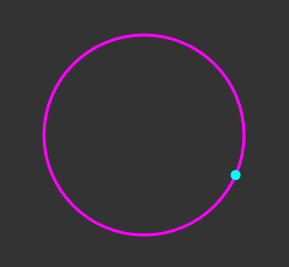
\includegraphics[width=0.4\textwidth]{images/bead.png}\\
圆上的珠子仿真效果
\end{center}


\vspace{\baselineskip}

\textbf{\fs{15}2. 双摆系统}

\begin{itemize}[leftmargin=2em, label={}]

\item 仿真效果和对应代码见 \texttt{hw4\_double\_pendulum.html}。\\
浏览器(推荐使用 Chrome)打开可查看动画,文本编辑器打开可查看代码。\\[-4ex]

\begin{center}
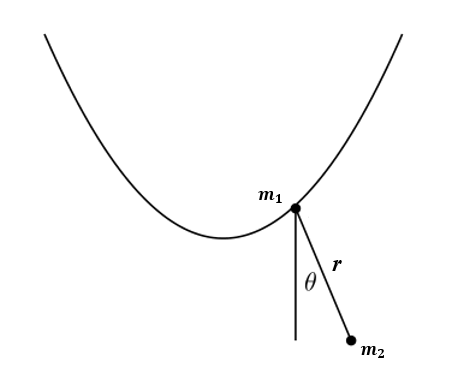
\includegraphics[width=0.4\textwidth]{images/parabola_x.png}\\
其中一个质点在抛物线上的双摆
\end{center}

\vspace{\baselineskip}

\setlength{\abovedisplayskip}{3pt}
\setlength{\belowdisplayskip}{3pt}
% \setlength{\abovedisplayshortskip}{0pt}
% \setlength{\belowdisplayshortskip}{0pt}

令 $(x_i,y_i)$ 表示质点 $m_i$ 的坐标,可以建立参数方程如下:
\begin{align*}
x_1 &= u \\
y_1 &= a\cdot u^2 \\
x_2 &= u + r\cdot \sin(\theta) \\
y_2 &= a \cdot u^2 - r\cdot \cos(\theta) \\
\end{align*}

对上述各式求一阶导数
\begin{align*}
x_1 &= \dot{u} \\
y_1 &= 2a\cdot u \cdot \dot{u} \\
x_2 &= \dot{u} + r\cdot \cos(\theta) \cdot \dot{\theta} \\
y_2 &= 2a \cdot u \cdot \dot{u} + r\cdot \sin(\theta) \dot{\theta} \\
\end{align*}

双摆系统的动能为
\begin{align*}
T &= \frac{1}{2} m_1 (\dot{x}^2_1 + \dot{y}^2_1) + \frac{1}{2} m_2 (\dot{x}^2_2 + \dot{y}^2_2)\\
  &= \frac{1}{2} (m_1+m_2) (1+4a^2u^2) \dot{u}^2 + \frac{1}{2} m_2 r^2 \dot{\theta}^2 + m_2 r \dot{u} \dot{\theta}(\cos(\theta)+2au\sin(\theta))
\end{align*}

双摆系统的势能为
\begin{align*}
V &= m_1 g y_1 + m_2 g y_2 \\
  &= (m_1+m_2)gau^2-mgr\cos(\theta)
\end{align*}

则拉格朗日量为
\begin{align*}
L = T - V
\end{align*}

只保留平方项
\begin{align*}
L = \frac{1}{2} (m_1+m_2) \dot{u}^2 + \frac{1}{2}m_2r^2\dot{\theta}^2 + m_2r\dot{u}\dot{\theta} - (m_1+m_2)gau^2 - \frac{1}{2} m_2 g r \theta^2
\end{align*}

则有对应的欧拉-拉格朗日方程,化简得到
\begin{align*}
& \ddot{u} + \frac{m_2}{m_1+m_2}r\ddot{\theta}+2gau=0 \\
& \ddot{u}+r\ddot{\theta} + g\theta=0
\end{align*}

进一步化简得到 $\ddot{u}$ 和 $\ddot{\theta}$ 的表达式
\begin{align*}
&\ddot{u} = -\frac{m_1+m_2}{m_1}\cdot 2gau+\frac{m_2}{m_1}\cdot gw \\
&\ddot{\theta} = \frac{m_1+m_2}{m_1r} \cdot (2gau-g\theta)
\end{align*}

\vspace{0.5\baselineskip}

使用四元四阶龙格-库塔方法进行数值模拟:
\vspace{\baselineskip}

\begin{lstlisting}[style=myC]
function uw2uwdd(u,w) {
    return [-(1+m2/m1)*2*g*a*u + m2/m1*g*w, (m1+m2)/(m1*r)*(2*g*a*u-g*w)];
}
// [udd,wdd,ud,wd] = f(ud,wd,u,w)
function f(ud,wd,u,w) {
    let [udd,wdd] = uw2uwdd(u,w);
    return [udd,wdd,ud,wd];
}
function rk(ud,wd,u,w) {
    let k1 = f(ud,wd,u,w);
    let tmp1 = add([ud,wd,u,w], mult(k1,h/2));
    let k2 = f(...tmp1);
    let tmp2 = add([ud,wd,u,w], mult(k2,h/2));
    let k3 = f(...tmp2);
    let tmp3 = add([ud,wd,u,w], mult(k3,h));
    let k4 = f(...tmp3);
    return add([ud,wd,u,w], mult(add(k1,mult(2,k2),mult(2,k3),k4),h/6));
}
function uw2xy1(u,w){
    return [u, -a*u*u];
}
function uw2xy2(u, w){
    return [u + r*sin(w), -a*u*u + r*cos(w)];
}

[ud,wd,u,w] = rk(ud,wd,u,w);
p1 = uw2xy1(u,w);
p2 = uw2xy2(u,w);
\end{lstlisting}
\end{itemize}

\begin{center}
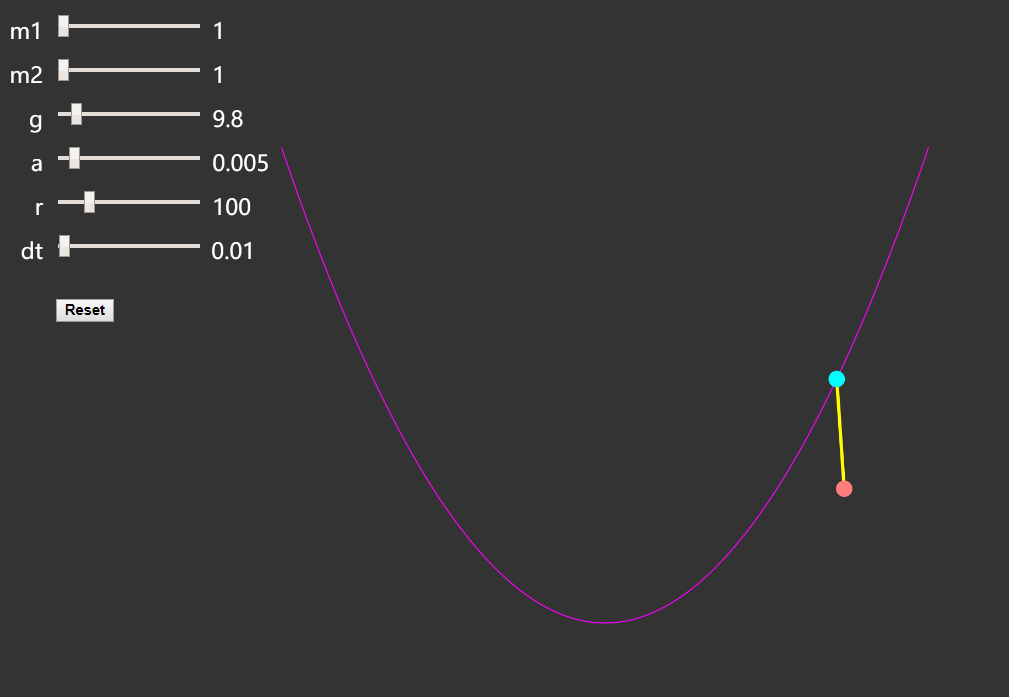
\includegraphics[width=0.85\textwidth]{images/pendulum.png}\\
抛物线上的双摆系统仿真效果
\end{center}



\end{document}